
\section{Introduction}

Recent technological advances allow unbiased investigation of cellular
dynamic processes in a high-throughput manner
 \cite{tanay_scalingsinglecellgenomics_2017,etzrodt_quantitativesinglecellapproaches_2014}.
Trajectory inference (TI) methods aim to give insight into a dynamic
process by inferring a trajectory from omics profiles of cells in which
the dynamic process takes place
 \cite{cannoodt_computationalmethodstrajectory_2016}. In a recent study,
we benchmarked 45 TI methods in terms of their accuracy, scalability,
stability, and
robustness \cite{saelens_comparisonsinglecelltrajectory_2019}. We
construct a set of guidelines to help end-users select an appropriate TI
method for their dataset of interest. However, executing and comparing
multiple methods remains challenging, due to high variability in
input/output data structures, software requirements, and programming
interfaces.

We developed {dyno}, a toolkit to easily infer, visualise and
interpret single-cell trajectories. The user can select the most optimal
set of TI methods based on characteristics of the dataset and user
preferences. More than 50 TI methods can easily be run within a common
interface, and the outputs thereof are converted into a common format.
{dyno} provides downstream analysis such as: visualising a
trajectory in a low-dimensional space or a heatmap, detecting genes
differentially expressed at different stages of the tragectory,
comparing multiple trajectories in a common dimensionality reduction,
and manipulating the trajectory such as adding directionality or
labelling different cell stages.

\section{Results}
This section will present the various components in the {dyno} workflow (Figure \ref{fig:dyno_toolkit}).

\begin{figure}[htb!]
	\centering
	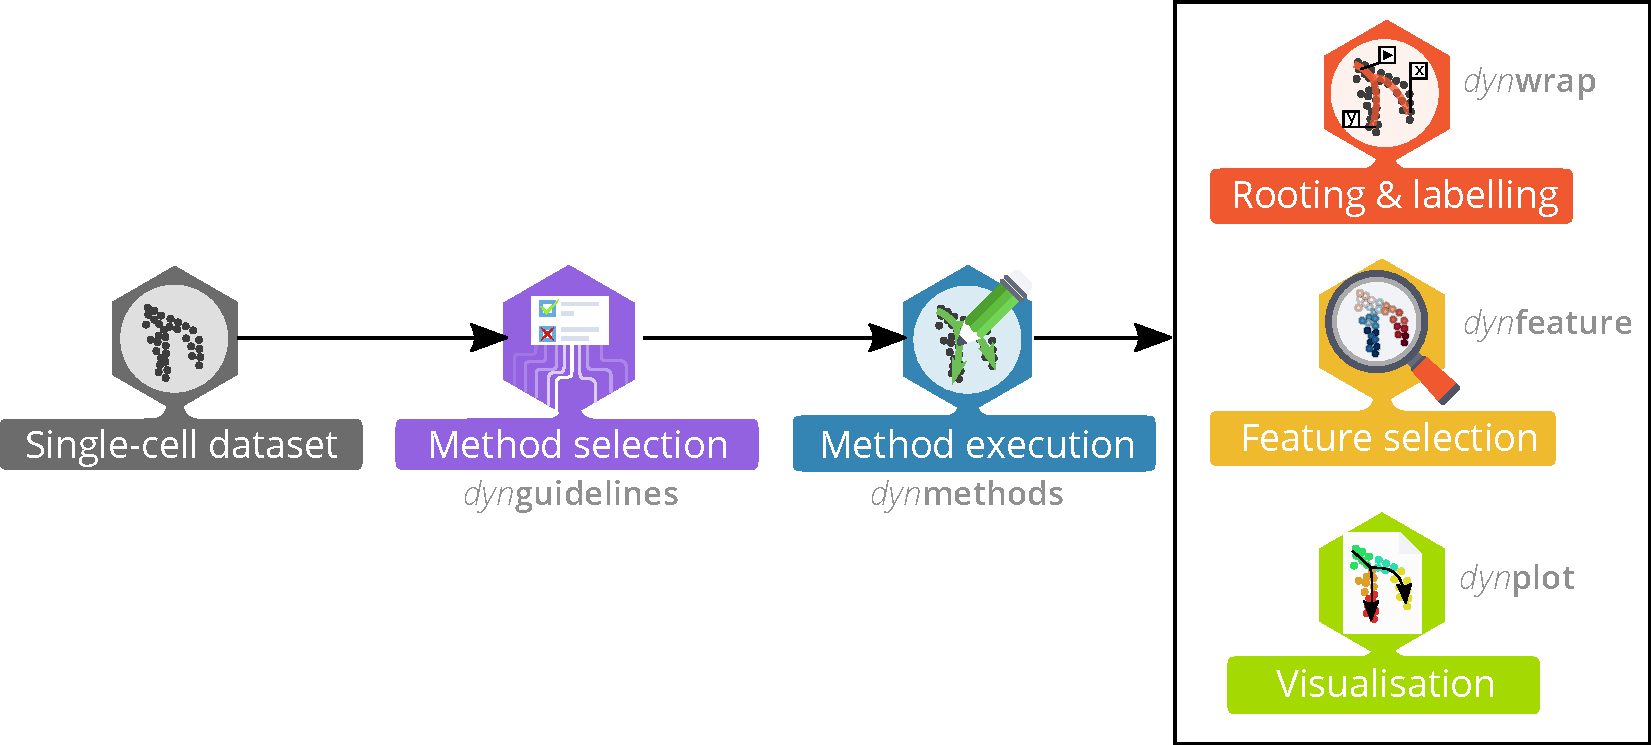
\includegraphics[width=.8\linewidth]{fig/toolkit.pdf}
	\caption{
		\textbf{The {dyno} workflow for inferring, visualising and interpreting single-cell trajectories.}
		{dynguidelines} allows you to choose a suitable TI method for your dataset of interest.
		{dynmethods} contains wrappers for `r dynmethods::methods %>% filter(method_source != "control") %>% nrow()` TI methods.
		{dynwrap} provides main functionality for (pre/post-)processing trajectory data structures.
		{dynfeature} calculates gene importance scores based on a trajectory.
		{dynplot} provides visualisation tools for trajectories, including scatterplots and heatmaps.
	}
	\label{fig:dyno_toolkit}
\end{figure}

\subsection{Preparing the dataset}
In order to use your dataset of interest, you will first need to wrap it in a {dynwrap} object. We will use a commonly used dataset of 392 mouse embryonic fibroblasts (MEF) undergoing direct reprogramming to induced neuronal cells \cite{treutlein_dissectingdirectreprogramming_2016}. By wrapping the counts information and possible prior information (e.g. known cell types, a start cell, time course information) into a {dynwrap} object, the dataset can be used as input for the various {dyno} components.

\subsection{Selecting the best methods for a dataset}

We performed a comparative study of 45 trajectory inference
methods \cite{saelens_comparisonsinglecelltrajectory_2019}. We evaluated
each method in terms of four main aspects:

\begin{itemize}
	\tightlist
	\item \textbf{Accuracy}: How similar is the inferred trajectory to the
	``true'' (or ``expected'') trajectory in the data. We used several
	metrics in order to assess similarity in pairwise cellular ordering
	and also the similarity in topology of the trajectories. We used both
	real datasets -- which has the highest biological relevance -- and
	synthetic datasets -- which allow to push methods to their limits more
	easily.
	\item \textbf{Scalability}: How long the method takes to run and how much
	memory it consumes. This mainly depends on the dimensions of the input
	data, i.e.~the number of cells and features.
	\item \textbf{Stability}: How stable the results are when rerunning the
	method with slightly different input data.
	\item \textbf{Usability}: The quality of the corresponding documentation,
	software package, and manuscript. We assessed how easy it is to run
	the method, whether the software adheres to good software development
	practices, and whether the manuscript follows good scientific
	practices. We reviewed `good practices' literature and created a
	`consensus' score-sheet of good practices, and filled in to what extent
	each method adhered to each of the good practices.
\end{itemize}

We found a high diversity in method performance, and that not many
methods perform well across the board. The performance of a method
depended on many factors, mainly the dimensions of the data and the kind
of trajectory present in the data. Based on this, we developed an
interactive Shiny \cite{rstudio_webapplicationframework_2016} app which can be used to explore the results and
select an optimal set of methods for a particular analysis
(Figure \ref{fig:dynguidelines_interface}).

\begin{figure}[htb!]
	\centering
	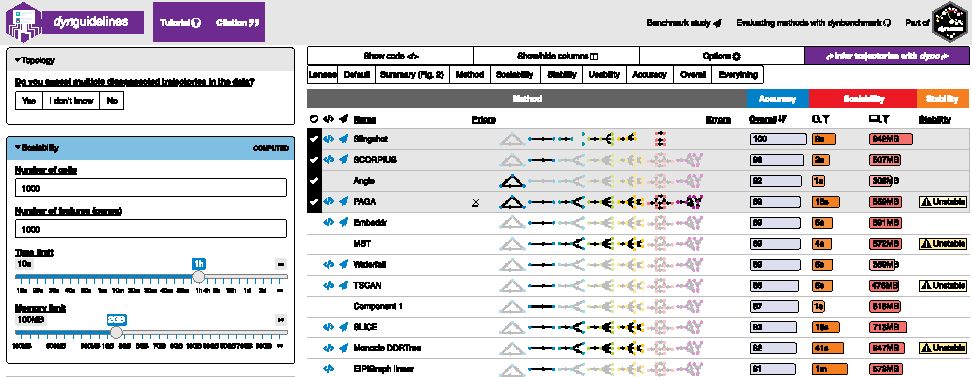
\includegraphics[width=\linewidth]{fig/shiny.pdf}
	\caption{\textbf{A static screenshot of the {dynguidelines} Shiny interface.}}
	\label{fig:dynguidelines_interface}
\end{figure}


\subsection{Inferring trajectories}
There are over 50 TI methods available as part of {dynmethods}, and executing a TI method on a dataset of interest is as simple as running just one command.
Behind the screens, {dyno} will save the dataset, prior
information and parameters as an H5 file and execute a container containing
the desired TI method. This
ensures that the TI method will not have any issues due to software
compatibilities on the host environment. The first time a TI method is
run, it will automatically download the corresponding container from
Docker Hub.

We inferred a trajectory on the dataset of mouse embryonic fibroblasts using the Slingshot \cite{street_slingshotcelllineage_2018} approach. The outputted model contains the main information on the trajectory, namely the milestone network and cell progressions (Table~\ref{tab:trajdata}). These data are hard to interpret manually. Luckily, {dyno} provides many different visualisation functions for interpreting trajectories.

\begin{table}
	\caption{The minimum amount of information to define a trajectory.}\label{tab:trajdata}
	\hfill
	\begin{minipage}[t]{.4\linewidth}
		\footnotesize
		\textbf{Milestone network:}

		\begin{tabular}{llrl}
			\toprule
			from & to & length & directed\\
			\midrule
			5 & 1 & 13.828399 & TRUE\\
			1 & 2 & 4.853443 & TRUE\\
			2 & 3 & 11.325468 & TRUE\\
			2 & 4 & 14.022826 & TRUE\\
			\bottomrule
		\end{tabular}
	\end{minipage}
	\hfill
	\begin{minipage}[t]{.4\linewidth}
		\footnotesize
		\textbf{Cell progressions:}

		\begin{tabular}{lllr}
		\toprule
		cell\_id & from & to & percentage\\
		\midrule
		1\_iN1\_C04 & 2 & 3 & 0.3508990\\
		1\_iN1\_C05 & 2 & 3 & 0.5287099\\
		1\_iN1\_C07 & 1 & 2 & 0.1953806\\
		1\_iN1\_C08 & 2 & 3 & 0.8589863\\
		1\_iN1\_C09 & 1 & 2 & 0.9076217\\
		1\_iN1\_C10 & 1 & 2 & 0.4170644\\
		1\_iN1\_C11 & 2 & 3 & 0.7316277\\
		1\_iN1\_C12 & 1 & 2 & 0.7108862\\
		1\_iN1\_C13 & 1 & 2 & 0.0644059\\
		1\_iN1\_C14 & 1 & 2 & 0.7178277\\
		\multicolumn{4}{c}{\ldots} \\
		\bottomrule
		\end{tabular}
	\end{minipage}
	\hfill\
\end{table}

\subsection{Execution details}

\paragraph{Prior information:} The method will error if it requires some prior information that is not
already provided in the dataset. Take note that the stronger the assumed priors for a given method, the more biased the output will be (Table~\ref{tab:prior}).

\begin{table}
	\caption{Possible prior information accepted or required by TI methods.}\label{tab:prior}
	\footnotesize
	\begin{tabularx}{\linewidth}{lXl}
		\toprule
		Name & Description & Type\\
		\midrule
		Start cell(s) & One or more start cell identifiers & soft\\
	  End cell(s) & One or more end cell identifiers & soft\\
		\# end states & The number of end states & soft\\
		\# start states & The number of start states & soft\\
		\# leaves & The number of leaves & soft\\
		\addlinespace
		Cell clustering & Named character vector linking the cell identifiers to different states/branches & hard\\
		\# states & Number of states/branches, including start, end and intermediary states & soft\\
		State network & Dataframe containing the known network between states/branches. Contains a from and to column & hard\\
		Time course (continuous) & Named numeric vector linking the cell ids to time points & hard\\
		Time course (discrete) & Named numeric vector linking the cell ids to time course points & hard\\
		\addlinespace
		Marker genes & Genes/features known to be important in the dynamic process & soft\\
		\bottomrule
	\end{tabularx}
\end{table}

\paragraph{Reproducibility:} When using this framework for analysing real data, remember to set the seed to ensure reproducibility.


\paragraph{Multiple executions:} Often it is useful to run multiple methods and/or use multiple datasets. While you can easily parallelise this yourself, we provide a helper
function which integrates well with our visualisation functions.

\paragraph{Errors:} Some methods can generate errors which are beyond our control. To know
what and where a method generated an error, remember to turn on the verbosity.

\paragraph{Command-line:} Each method is also executable from command-line using the Docker container. Check out the help documentation by running a TI method container without extra arguments.




\subsection{Visualising trajectories}

The most common way to visualise a trajectory is to plot it on a
dimensionality reduction of the cells (Figure~\ref{fig:dimred}A).
Often (but not always), a TI
method will already output a dimensionality reduction itself, which was
used to construct the trajectory. {dynplot} will use this
dimensionality reduction if available, otherwise it will calculate a
dimensionality reduction under the hood.
You can also supply it with your own dimensionality reduction. In this
case, the trajectory will be \emph{projected} onto this dimensionality
reduction (Figure~\ref{fig:dimred}B).
On this plot, you can colour the cells using various layers of information (Figure~\ref{fig:colorby}): cell ordering, cell grouping, feature expression, and pseudotime.


\begin{figure}[ht!]
  \centering
  A
  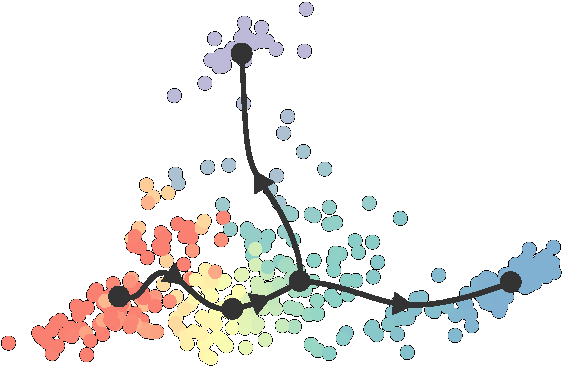
\includegraphics[width=.4\linewidth,valign=t]{manuscript_files/figure-latex/plotslingshot-1.pdf}
  B
  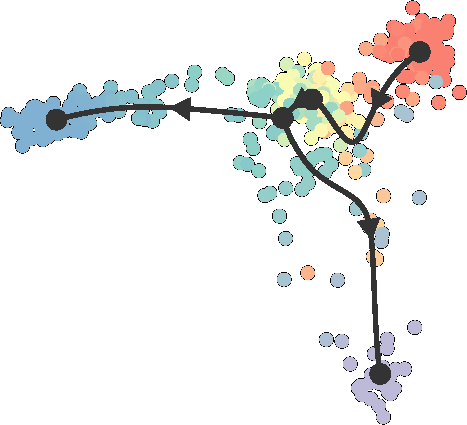
\includegraphics[width=.4\linewidth,valign=t]{manuscript_files/figure-latex/plotslingshot_umap-1.pdf}
  \caption{
  	\textbf{A:} Often, the TI method provides its own dimensionality reduction for the trajectory, which will be plotted by default. This is a visualisation of Slingshot \cite{street_slingshotcelllineage_2018} executed on MEF cells from the previous example.
  	\textbf{B:} Alternatively, you can provide your own dimensionality reduction, and the trajectory will be projected to it. In this example the Slingshot trajectory is projected to a UMAP dimensionality reduction \cite{mcinnes_umapuniformmanifold_2018}.
	}
\label{fig:dimred}
\end{figure}

\begin{figure}[ht!]
	\centering
	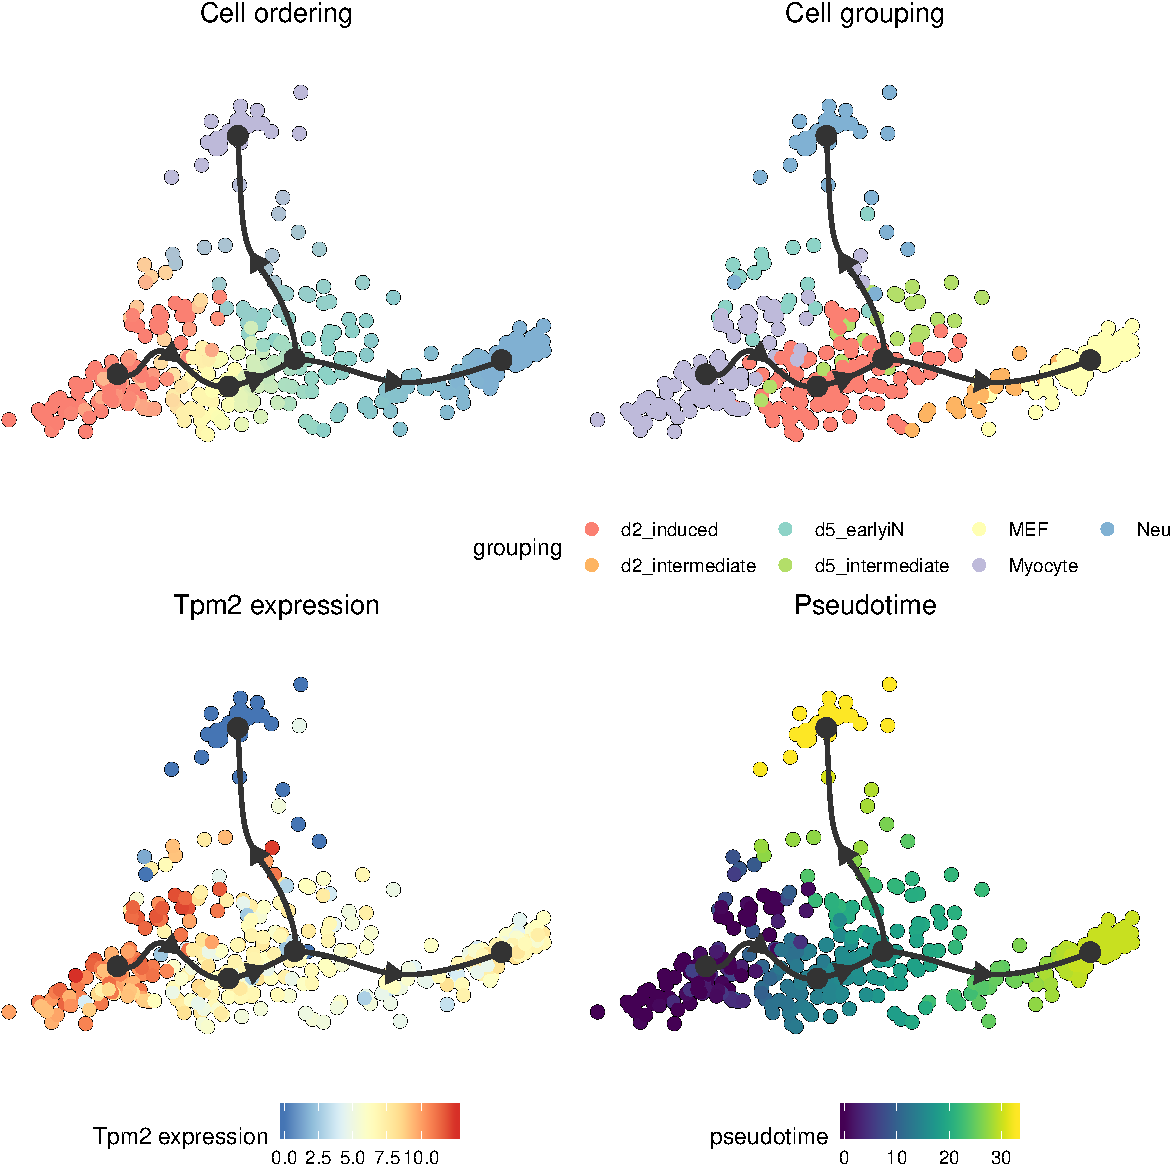
\includegraphics[width=.6\linewidth]{manuscript_files/figure-latex/slingshot_multi-1.pdf}
  \caption{
		\textbf{Cell ordering:} Cells are coloured by their proximity to the different milestones.
		\textbf{Cell grouping:} A given character vector mapping a cell to a group.
		\textbf{Feature expression:} Colour by the expression levels of a particular gene.
		\textbf{Pseudotime:} The distance to a particular root milestone.
	}
	\label{fig:colorby}
\end{figure}


\paragraph{Various layout and colouring options:} To visualise a trajectory, it is good practice to take into account what the purpose and intended message of the visualisation is (Figure~\ref{fig:cells}).
The cells and trajectory can be positioned to place more emphasis on the topology of the inferred trajectory, or on the cellular heterogeneity between the cells, that the trajectory might or might not have been able to detect. Cells and trajectory can be coloured according to the
topology of the trajectory, according to gene expression, or a custom
input vector of values.

\begin{figure}[ht!]
	\centering
	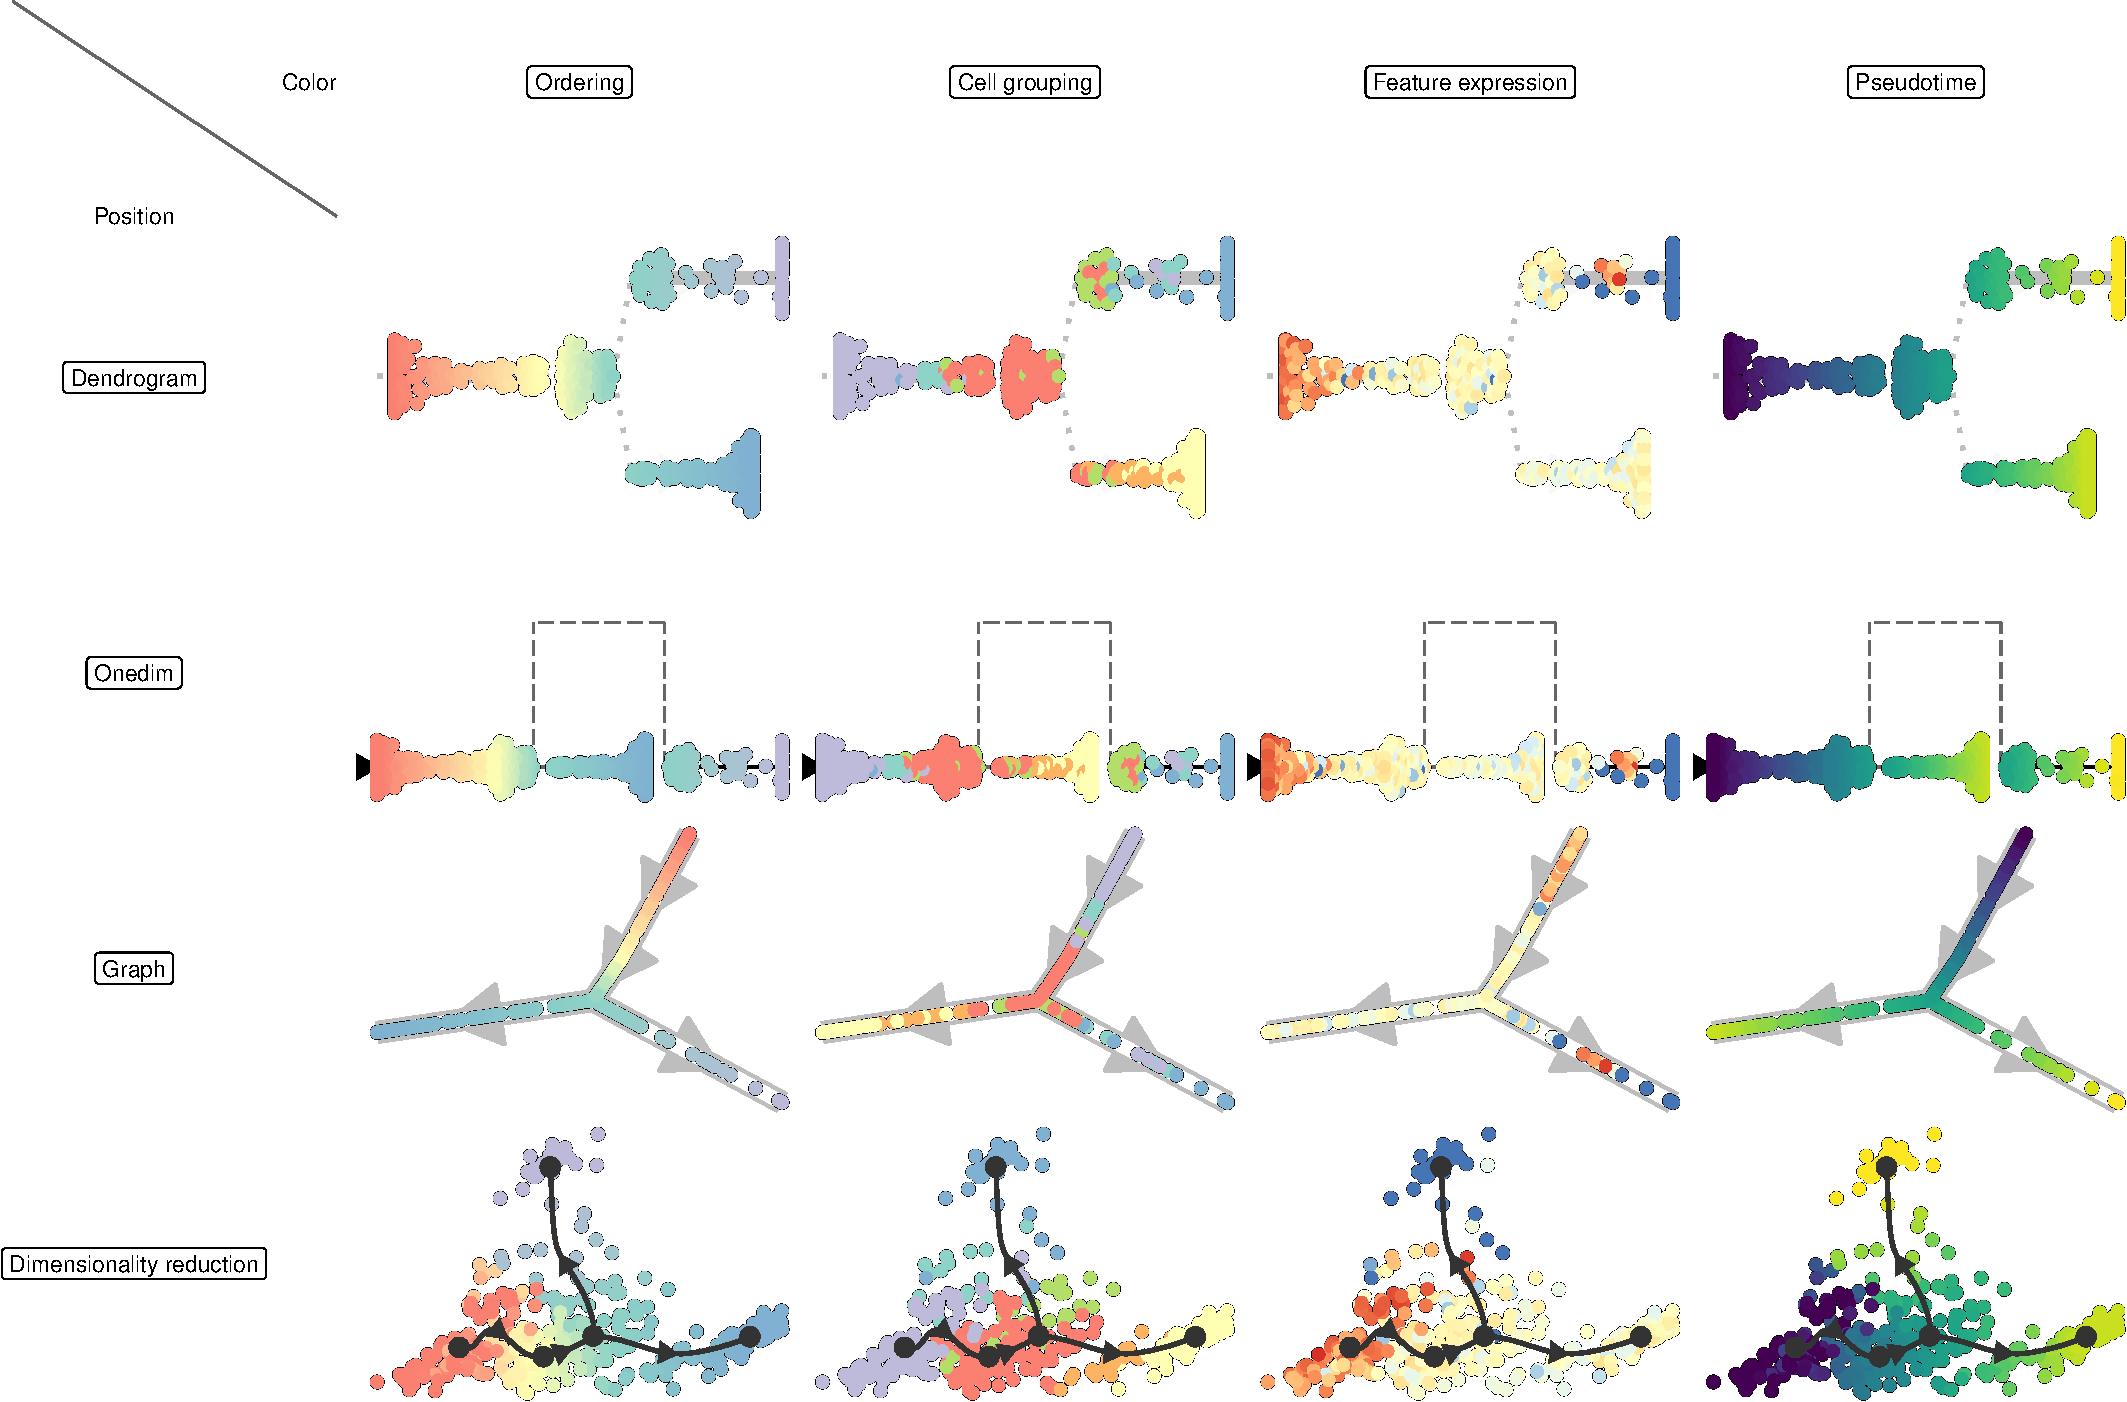
\includegraphics{manuscript_files/figure-latex/cells-1.pdf}
	\caption{Overview of the different combinations of positioning and
		colouring options, demonstrated on the output of Slingshot \cite{street_slingshotcelllineage_2018}.}
	\label{fig:cells}
\end{figure}


\paragraph{Visualising many genes along a trajectory:}
A one-dimensional visualisation is especially useful if you combine it
with a heatmap (Figure~\ref{fig:heatmap}).

\begin{figure}[ht!]
	\centering
	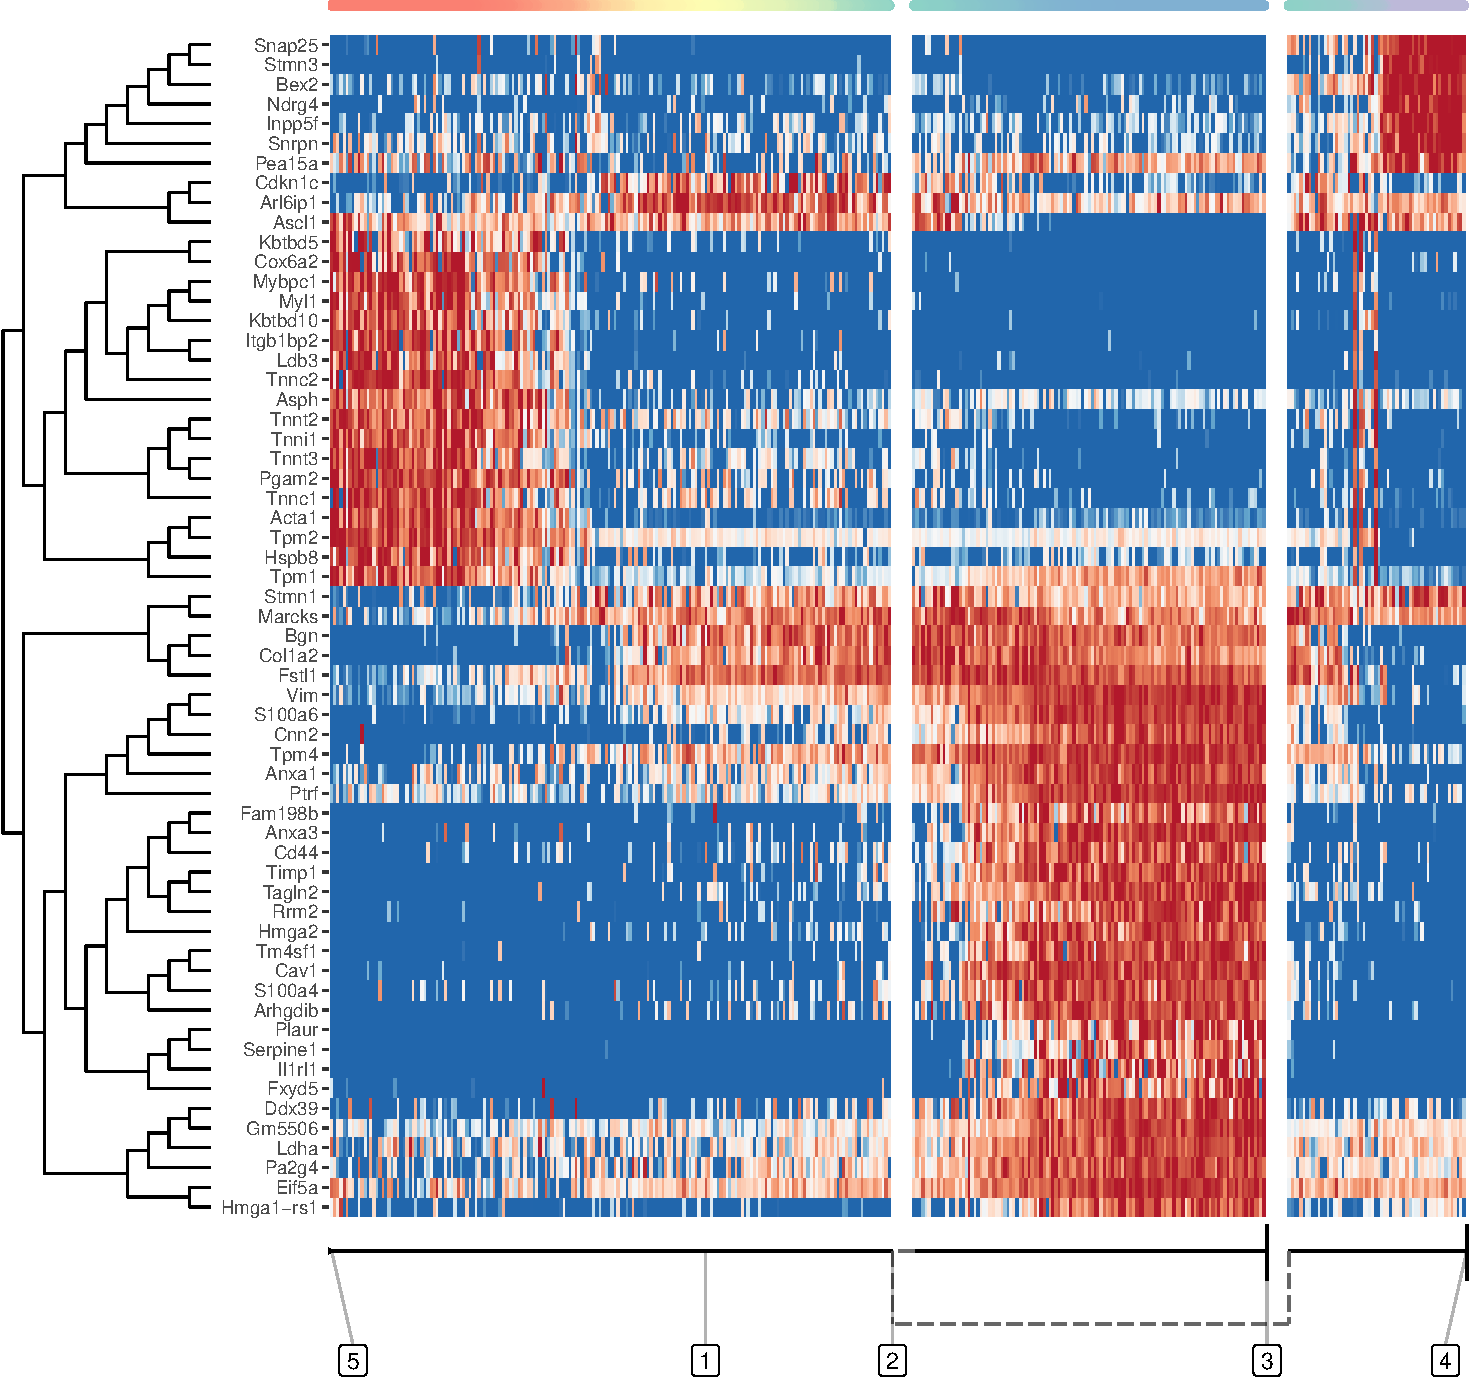
\includegraphics[width=.6\linewidth]{manuscript_files/figure-latex/heatmap-1.pdf}
	\caption{Selecting relevant features for this heatmap is discussed in a later
		section, By default, features will be selected that best explain the main differences over the
		whole trajectory.}
	\label{fig:heatmap}
\end{figure}


\paragraph{Comparing multiple trajectories:}
Visualising each method with
their own dimensionality reduction can make it hard to interpret to what
extend the methods agree/disagree with each-other (Figure~\ref{fig:compare}A).
Different trajectories become noticeably more comparable when projected
to a common dimensionality reduction (Figure~\ref{fig:compare}B).

\begin{figure}[ht!]
	\centering
	\textbf{A}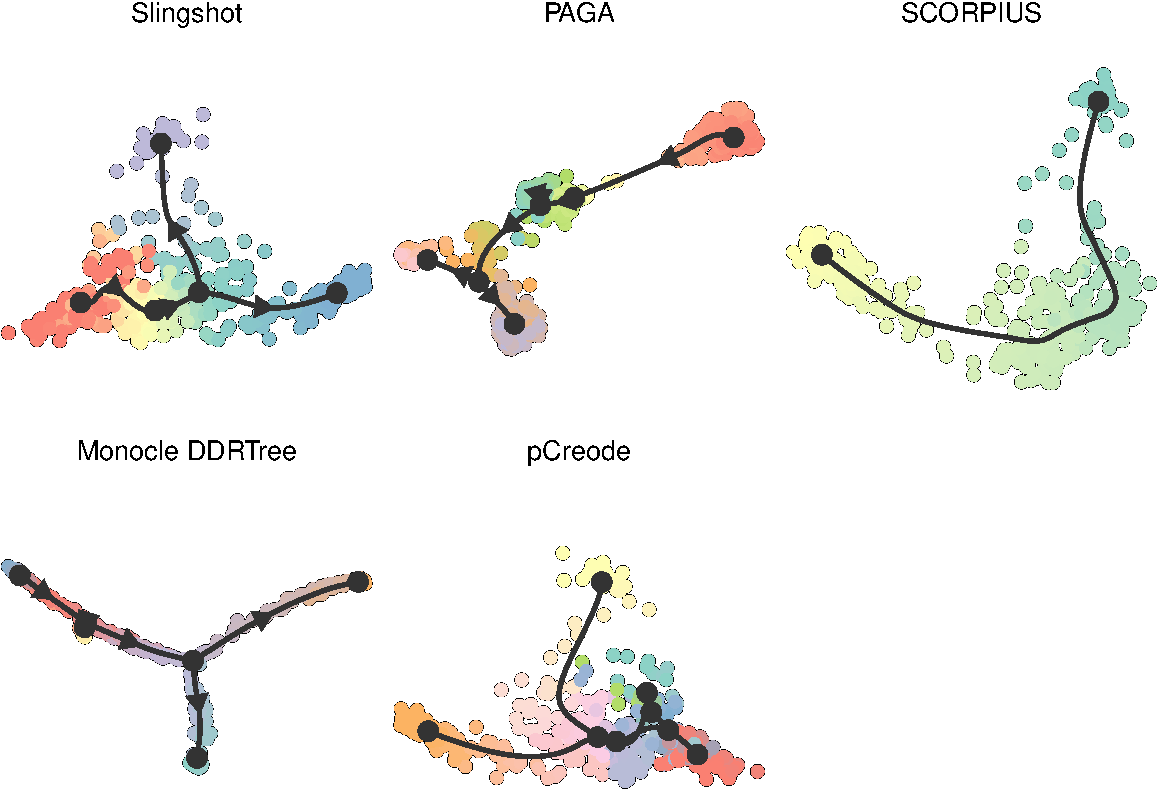
\includegraphics[width=.6\linewidth,valign=t]{manuscript_files/figure-latex/dimreds-1.pdf}\\\vspace*{1em}
	\textbf{B}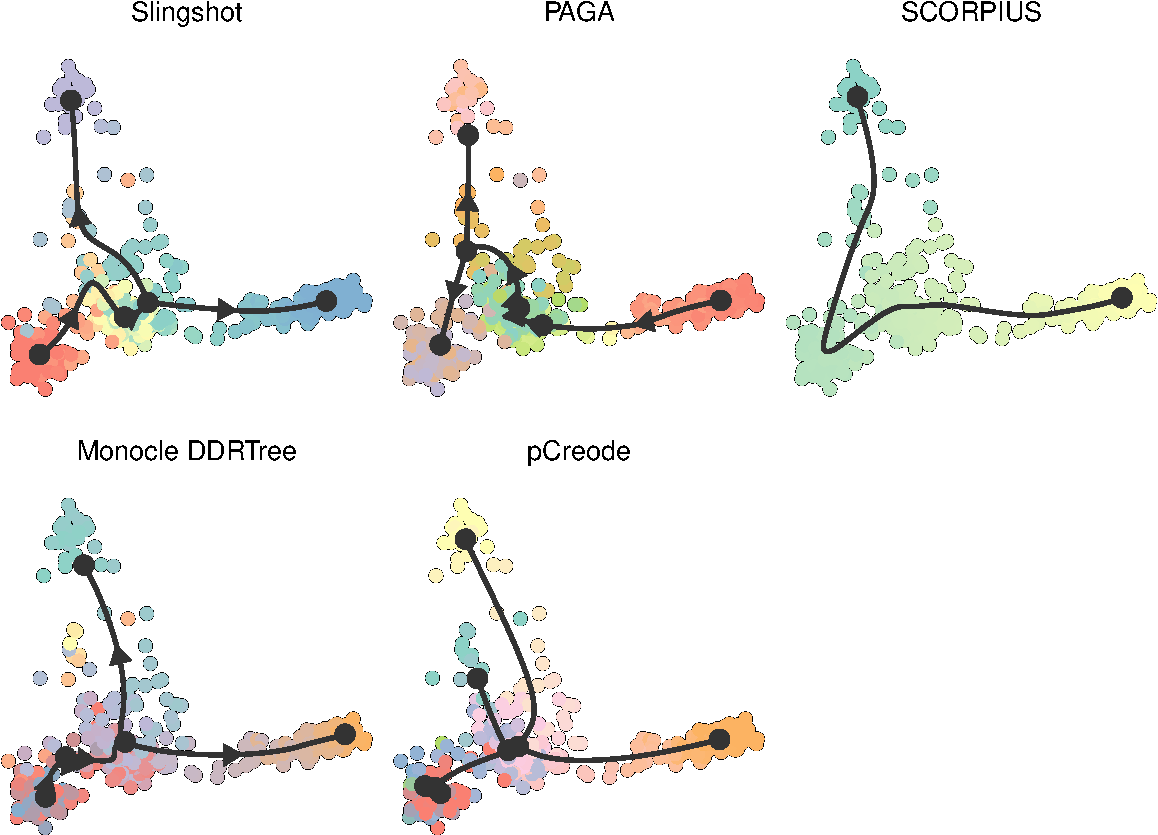
\includegraphics[width=.6\linewidth,valign=t]{manuscript_files/figure-latex/dimredscommon-1.pdf}
	\caption{
		\textbf{A:} Comparing outputs of multiple TI methods is tedious when they are each visualised using their own visualisation method of interest.
		\textbf{B:} In contrast, by projecting each output to the same dimensionality reduction, the methods become immediately visually comparable.
	}
	\label{fig:compare}
\end{figure}






\subsection{Manipulating the trajectory}
{dyno} allows manipulating trajectories by simplifying, rooting and annotating them.

\paragraph{Simplifying linear segments:} Intermediate milestones can be removed by simplifying the trajectory (Figure~\ref{fig:annot}A).


\begin{figure}[ht!]
	\centering
	\textbf{A}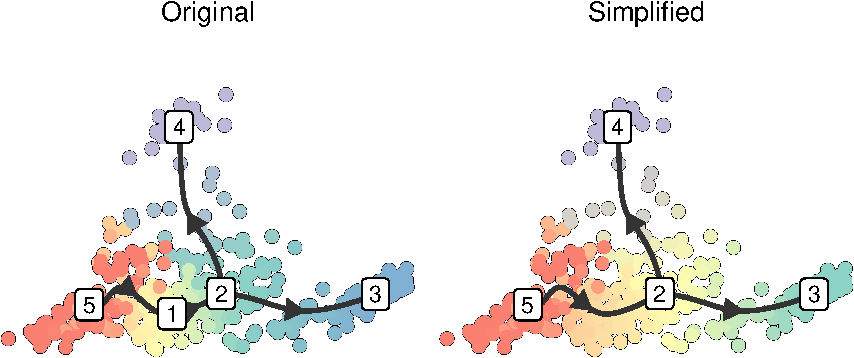
\includegraphics[width=.7\linewidth,valign=t]{manuscript_files/figure-latex/unnamed-chunk-31-1.pdf} \\
	\textbf{B}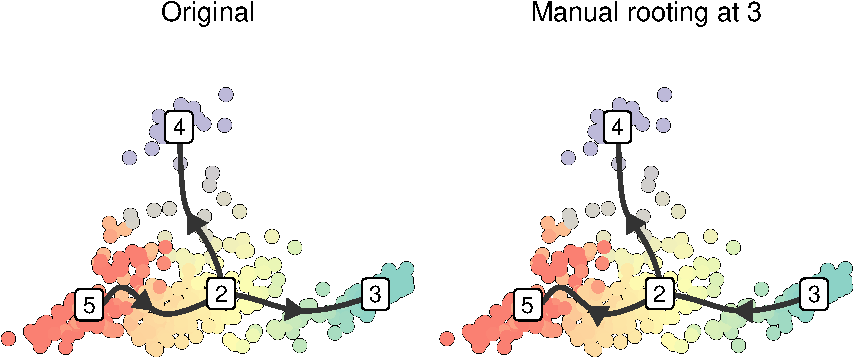
\includegraphics[width=.7\linewidth,valign=t]{manuscript_files/figure-latex/rootmanual-1.pdf}\\
	\textbf{C}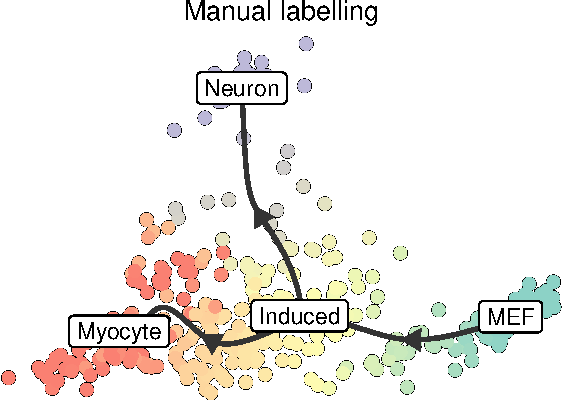
\includegraphics[width=.35\linewidth,valign=t]{manuscript_files/figure-latex/annotatemanual-1.pdf}
	\caption{
		\textbf{A:} Simplification of the trajectory.
		\textbf{B:} Rooting the trajectory.
		\textbf{C:} Labelling the trajectory.
	}
	\label{fig:annot}
\end{figure}




\paragraph{Rooting:} Most TI methods return undirected trajectories. We provide two ways of
rooting a trajectory, namely by manually specifying the root milestone, or by specifying highly expressed marker genes. After rooting, all other edges will point away from the root (Figure~\ref{fig:annot}B).


\paragraph{Annotating the trajectory:} Similar as with rooting, annotating the trajectory by renaming the
milestones can be done either manually, or with given highly expressed
gene sets (Figure~\ref{fig:annot}C).





\subsection{Differentially expressed genes along the trajectory}

Compared to differential expression between clusters of cells, defining
differential expression on trajectories is not so straightforward. What
constitutes a trajectory differentially expressed gene?

\begin{itemize}
\tightlist
\item A gene that is uniquely expressed in a particular branch?
\item A gene that changes at a branching point?
\item A gene that changes along pseudotime?
\end{itemize}

{dynfeature} allows you to find these different kinds of
differential expression in a trajectory. It first defines a particular
variable that needs to be predicted (for example, whether a cell is
present in a branch or not), and ranks each gene based on their
predictive capability with respect to that variable. This section
reviews the types of feature selection supported by {dynfeature}.


\paragraph{Lineage / transition marker genes:}
We can identify genes that are specifically upregulated or downregulated
at a specific branch (Figure~\ref{fig:fimp_tran}).

\begin{figure}
{\footnotesize
\begin{tabular}{lllr}
\toprule
feature\_id & from & to & importance\\
\midrule
Cav1 & 3 & 2 & 3.289198\\
S100a6 & 3 & 2 & 2.942703\\
1810020D17Rik & 2 & 5 & 2.822247\\
Tagln2 & 3 & 2 & 2.763266\\
Bex2 & 2 & 4 & 2.672312\\
\addlinespace
Anxa3 & 3 & 2 & 2.630013\\
Tm4sf1 & 3 & 2 & 2.547472\\
Vim & 3 & 2 & 2.431169\\
Hmga2 & 3 & 2 & 2.376114\\
Rrm2 & 3 & 2 & 2.346754\\
\bottomrule
\end{tabular}
}
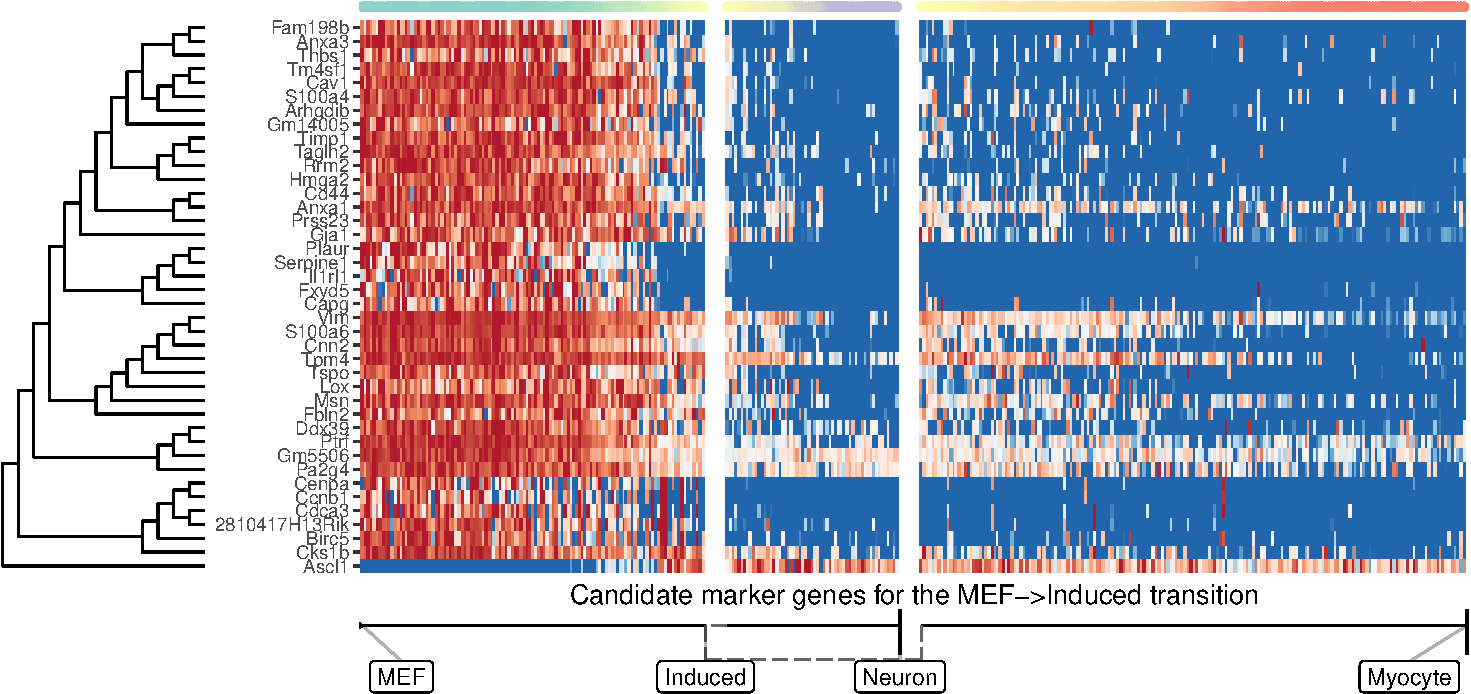
\includegraphics[width=.6\linewidth,valign=m]{manuscript_files/figure-latex/branchheatmap-1.pdf}
\caption{Candidate markers genes for the MEF $\rightarrow$ transition.}
\label{fig:fimp_tran}
\end{figure}

\paragraph{Milestone marker genes:}
We can identify genes that are specifically upregulated or downregulated
at a particular milestone (Figure~\ref{fig:fimp_mil}).

\begin{figure}
	{\footnotesize
\begin{tabular}{llr}
\toprule
milestone\_id & feature\_id & importance\\
\midrule
2 & S100a6 & 2.654416\\
2 & Cav1 & 2.567051\\
2 & Tagln2 & 2.501074\\
2 & Fam198b & 2.334142\\
2 & Timp1 & 2.056474\\
\addlinespace
2 & Anxa3 & 2.009431\\
2 & Tm4sf1 & 1.982274\\
2 & Vim & 1.833045\\
2 & Bex2 & 1.738471\\
2 & Rrm2 & 1.678349\\
\bottomrule
\end{tabular}
}
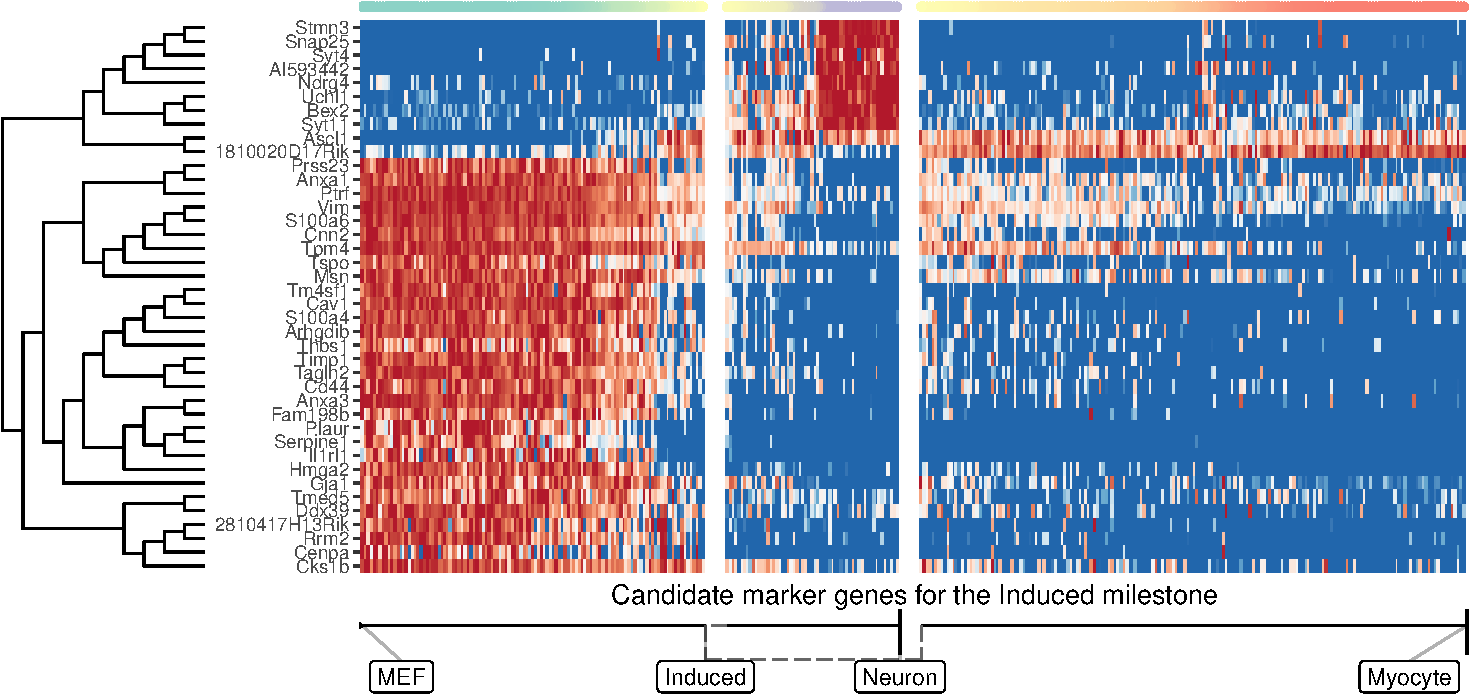
\includegraphics[width=.6\linewidth,valign=m]{manuscript_files/figure-latex/milestoneimpheatmap-1.pdf}
\caption{Candidate markers genes for the 'induced' milestone.}
\label{fig:fimp_mil}
\end{figure}


\paragraph{Marker genes for the trajectory as a whole:}
We can identify genes that change in function of the ordering of a part
of the trajectory (Figure~\ref{fig:fimp_over}).

\begin{figure}
\hfill
	{\footnotesize
\begin{tabular}{lr}
\toprule
feature\_id & importance\\
\midrule
Tpm2 & 0.4539798\\
Tagln2 & 0.3364078\\
Vim & 0.3319566\\
Plaur & 0.3252199\\
Cav1 & 0.3224918\\
\addlinespace
Hmga2 & 0.3189412\\
Ptrf & 0.3180152\\
Tnnc2 & 0.3092800\\
Acta1 & 0.3087145\\
Myl1 & 0.3014400\\
\bottomrule
\end{tabular}
}\hfill
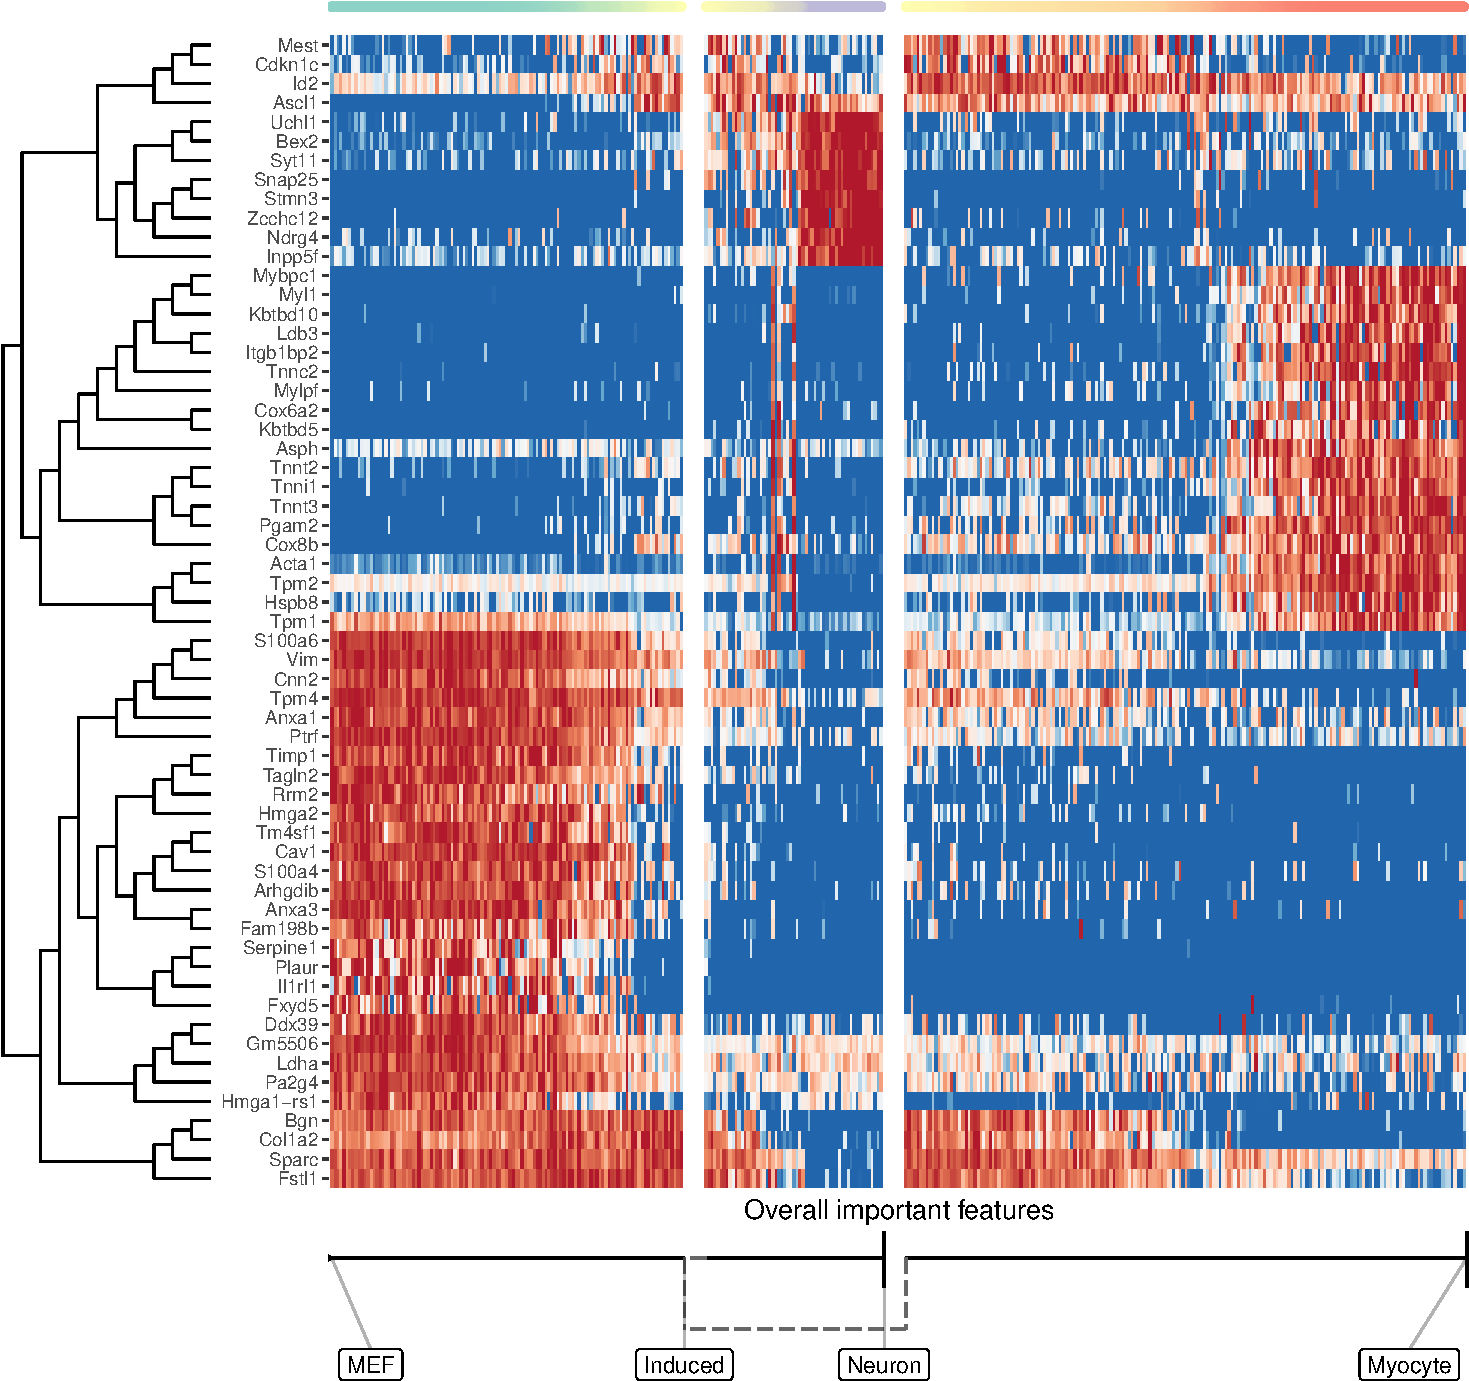
\includegraphics[width=.6\linewidth,valign=m]{manuscript_files/figure-latex/overallheatmap-1.pdf}
\caption{Candidate markers genes for the overall trajectory.}
\label{fig:fimp_over}
\end{figure}





\section{Discussion}
With {dyno}, we provide a feature-complete toolbox for inferring, visualising and annotating trajectory data. In this work, we demonstrated its usefulness by applying all of its visualisation and manipulation functionality on a particular dataset.

Alternative modalities such as ATAC-Seq or cytometry data are not yet
supported, although it is possible to simply include this data as
expression and counts.
RNA velocity \cite{lamanno_rnavelocitysingle_2018} would be particularly useful, as it would allow
rooting the directory without any further input from the user.

We are also planning to implement additional tools for interpreting the trajectories, such as alignment and differential expression. While the feature importance tools are incredibly useful towards interpreting trajectories, they do not yet provide a statistical ground to find features which are significantly
differentially expressed. In addition, depending on the size of the
dataset and of the predicted trajectory, it might take a long time to
compute.



